% ---------------------------------------------------------------
% 3.2  V-MARCH Overview
% ---------------------------------------------------------------
\subsection{\ours Overview}
\label{sec:overview}

\begin{figure*}[t]
    \centering
    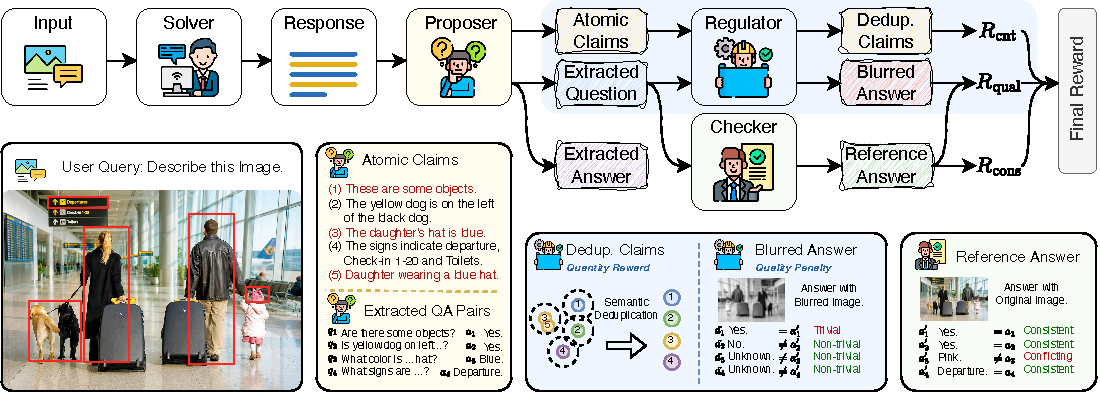
\includegraphics[width=\textwidth]{figures/v-march-pipeline2.pdf}
    \caption{Overview of the \ours pipeline.
    Given a \textbf{Solver}-generated response, the \textbf{Proposer} decomposes it into atomic factual claims and converts each into a visual question-answer pair.
    The \textbf{Regulator} performs Visual Claim Regulation (VCR) by deduplicating semantically redundant claims, rewarding claim quantity, and penalizing image-agnostic claims that can be answered without genuine visual perception.
    The \textbf{Checker} re-answers each question using the original image, and verifies consistency with the Solver's answers.
    The final self-verifying reward aggregates the Checker's consistency signal and the Regulator's quantity and quality signals.
    }
    \label{fig:pipeline}
\end{figure*}

\ours adapts the Proposer--Checker paradigm~\cite{wang2026visionzero,li2026march} to the visual domain and extends it with a dedicated \textbf{Regulator} agent.
The Regulator governs the quantity and quality of the claim set, addressing unreliable rewards to visual self-verification.
As illustrated in Figure~\ref{fig:pipeline}, \ours orchestrates four agents in a sequential pipeline:

\begin{itemize}[leftmargin=1em,itemsep=2pt]
\item \textbf{Solver.} Generates a response $y$ conditioned on the
    image--instruction pair $(I, q)$.
    Only the Solver is updated by GRPO training.
\item \textbf{Proposer.} Decomposes $y$ into a set of
    atomic factual claims $\mathcal{C} = \{c_1, \ldots, c_m\}$ and
    converts each claim into a visual question-answer pair, yielding the
    raw claim set $\mathcal{Q} = \{(v_i, a_i)\}_{i=1}^{m}$.
\item \textbf{Regulator.} Audits $\mathcal{Q}$ by
    (i)~removing semantically redundant claims to prevent reward inflation
    via repetition, yielding the filtered set
    $\mathcal{Q}^{\ast} = \{(v_i, a_i)\}_{i=1}^{n}$, $n \leq m$;
    (ii)~rewarding sufficient claim coverage via a claim-count signal
    $R_{\mathrm{cnt}}$; and (iii)~penalizing image-agnostic claims that
    can be resolved without genuine visual perception via a quality signal
    $R_{\mathrm{qual}}$. 
    We refer to the claim-level quantity and quality control as \textbf{Visual Claim Regulation} (VCR), which is described in detail in Section~\ref{sec:regulator}.
\item \textbf{Checker.} Receives the original image $I$ and questions $\{v_i\}$ from $\mathcal{Q}^{\ast}$, with no access to $y$.
    It generates image-grounded reference answers $\{a_i'\}$ and verifies
    consistency with the claim-implied answers $\{a_i\}$ via majority
    voting, producing a consistency reward $R_{\mathrm{cons}}$.
\end{itemize}

The final self-verifying reward aggregates signals from the Regulator and
the Checker:
\begin{equation}
    R_{\mathrm{SV}}(I, q, y)
    = \underbrace{R_{\mathrm{cons}}}_{\text{Checker}}
    + \underbrace{R_{\mathrm{cnt}} + R_{\mathrm{qual}}}_{\text{Regulator}}.
    \label{eq:reward_total}
\end{equation}
This reward is used directly as the GRPO training signal for the Solver,
requiring no human annotation or external supervision.

% This \emph{information asymmetry}---the Checker observes the image but not the generated description---breaks the self-confirmation bias inherent in single-model verification.


% ---------------------------------------------------------------
% 3.3  Proposer: Claim Extraction
% ---------------------------------------------------------------
\subsection{Proposer: Claim Extraction}
\label{sec:proposer}

Given $y$, the Proposer extracts a set of atomic factual
claims:
\begin{equation}
    \mathcal{C} = \{c_1, \ldots, c_m\} = \mathrm{Extract}(y),
\end{equation}
where each $c_i$ is a short, self-contained statement about a single visual
fact (e.g., object existence, color, quantity, or spatial relation).
Each claim is then converted into a visual question-answer pair:
\begin{equation}
    (v_i,\, a_i) = \mathrm{QA}(c_i),
    \qquad i = 1, \ldots, m,
\end{equation}
where $a_i$ is the answer implied by the claim.
The resulting raw claim set $\mathcal{Q} = \{(v_i, a_i)\}_{i=1}^{m}$
is passed to the Regulator for quality control before verification.


% ---------------------------------------------------------------
% 3.4  Regulator: Visual Claim Regulation
% ---------------------------------------------------------------
\subsection{Regulator: Visual Claim Regulation}
\label{sec:regulator}

The Regulator addresses three degenerate behaviors that undermine the
reliability of visual self-verification if left unchecked:
(1)~a model can repeat near-identical claims to inflate $R_{\mathrm{cons}}$;
(2)~it can produce very few but easily verified claims to obtain a stable
reward while remaining under-informative;
(3)~it can generate image-agnostic claims (e.g., \textit{``the image contains
objects''}) whose answers follow from language priors rather than genuine
visual perception.
The Regulator counteracts all three failure modes through semantic
deduplication and two complementary reward signals.

\paragraph{Semantic Deduplication.}
To address failure mode~(1), the Regulator removes semantically overlapping
claims from $\mathcal{Q}$ using cosine similarity over sentence embeddings
$\phi(\cdot)$:
\begin{equation}
    \mathrm{sim}(c_i, c_j)
    = \frac{\phi(c_i)^{\top} \phi(c_j)}
           {\|\phi(c_i)\| \cdot \|\phi(c_j)\|}.
\end{equation}
Pairs exceeding a type-aware similarity threshold are merged, yielding the
deduplicated claim set $\mathcal{Q}^{\ast} = \{(v_i, a_i)\}_{i=1}^{n}$,
$n \leq m$, which is forwarded to the Checker for verification.

\paragraph{Informativeness Reward.}
To address failure mode~(2), the Regulator adds a claim-count reward
proportional to the number of deduplicated claims $n$, capped at a target
$n_{\mathrm{target}}$:
\begin{equation}
    R_{\mathrm{cnt}}
    = \lambda_{\mathrm{cnt}}
      \cdot \min\!\left(\frac{n}{n_{\mathrm{target}}},\; 1\right),
\end{equation}
with $\lambda_{\mathrm{cnt}} = 0.5$ so that factual consistency remains
the dominant signal.
Because $n$ counts only deduplicated claims, failure modes~(1) and~(2)
are addressed jointly: repetition neither inflates $n$ nor contributes
to $R_{\mathrm{cnt}}$.

\paragraph{Visual-Dependence Penalty.}
To address failure mode~(3), the Regulator constructs a degraded image
$\tilde{I}$ by applying a heavy Gaussian blur, grayscale conversion, and
horizontal flipping to $I$.
It then re-answers each question $v_i$ in $\mathcal{Q}^{\ast}$ with the
degraded image:
\begin{equation}
    \tilde{a}_i = \mathrm{Ans}(\tilde{I},\, v_i).
\end{equation}
If $\tilde{a}_i$ remains consistent with the original reference answer
$a_i'$, the claim is marked trivial---i.e., answerable without meaningful
visual content:
\begin{equation}
    t_i = \mathbbm{1}\!\left[
        f_{\mathrm{ver}}(\tilde{a}_i,\, a_i') = 1
    \right].
\end{equation}
The Regulator penalizes trivial claims proportionally:
\begin{equation}
    R_{\mathrm{qual}} = -\lambda_{\mathrm{qual}} \sum_{i=1}^{n} t_i,
\end{equation}
pushing the Solver toward descriptions that require genuine image grounding.


% ---------------------------------------------------------------
% 3.5  Checker: Image-Grounded Verification
% ---------------------------------------------------------------
\subsection{Checker: Image-Grounded Verification}
\label{sec:checker}

The Checker receives the filtered claim set $\mathcal{Q}^{\ast}$ output by
the Regulator and the original image $I$, with no access to
$y$.
For each question $v_i \in \mathcal{Q}^{\ast}$, it generates an
image-grounded reference answer:
\begin{equation}
    a_i' = \mathrm{Ans}(I,\, v_i),
\end{equation}
and verifies consistency with the claim-implied answer via majority voting
over $K$ independent runs:
\begin{equation}
    z_i = \mathbbm{1}\!\left[
        \sum_{k=1}^{K} z_i^{(k)} > \frac{K}{2}
    \right],
    \qquad
    z_i^{(k)} = f_{\mathrm{ver}}(a_i,\, a_i').
\end{equation}
The resulting consistency reward is
\begin{equation}
    R_{\mathrm{cons}} = \frac{1}{n} \sum_{i=1}^{n} z_i,
\end{equation}
measuring the fraction of claims in $\mathcal{Q}^{\ast}$ that are supported
by image-grounded evidence.
This \emph{information asymmetry}---the Checker observes the image but not
the Solver's response---prevents the verifier from inheriting the same
hallucination tendencies as the generator, thereby producing a more reliable
consistency signal than single-model self-verification.

\paragraph{Final Reward.}
Combining the Checker and Regulator signals, the total reward used for
GRPO training is (cf.\ Eq.~\eqref{eq:reward_total}):
\begin{equation}
    R_{\mathrm{SV}}(I, q, y)
    = R_{\mathrm{cons}} + R_{\mathrm{cnt}} + R_{\mathrm{qual}}.
\end{equation}
The three terms are complementary: $R_{\mathrm{cons}}$ enforces factual
grounding; $R_{\mathrm{cnt}}$ promotes visual coverage; and
$R_{\mathrm{qual}}$ filters out image-agnostic claims.
Together, the four-agent pipeline provides a reliable, annotation-free
reward signal for scalable hallucination mitigation in VLMs.
